\section{Lab 3 - Complex Addition Systems}

\subsection{Introduction}
From your pocket calculator to inside modern CPUs adders have long been used as more than just a simple way to sum numbers together. This lab will go into the logic structure of the adder as well as provide a method for converting the simple full adder in to an \emph{arithmetic logic unit} (ALU) capable of handling 12 operations.

\subsection{Pre-lab}
Before coming to the lab, please complete the following and upload to Sakai:
\begin{itemize}
	\item A truth table for a half adder and a full adder
	\item The logic equation for a 4-bit ripple carry adder
\end{itemize}

\subsection{Lab Activities}

\subsubsection{Half Adder}
Build the circuit in Figure \ref{fig:halfadder}, create waveforms to verify that the logic is correct.

\begin{figure}[H]
	\centering
	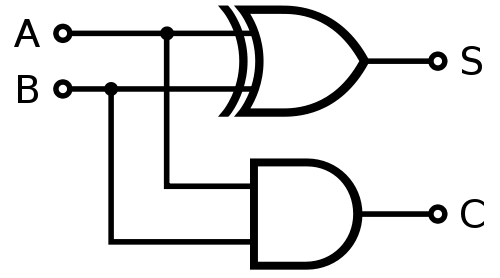
\includegraphics[width=60mm]{Lab3/figures/halfadder.png}
	\caption{Circuit for a 1-bit half adder}
	\label{fig:halfadder}
\end{figure}

\subsubsection{Full Adder}
The circuit in Figure \ref{fig:fulladder} implements a full 1-bit adder. Implement this circuit in VHDL, create a waveform, and verify that the logic behaves as expected. 

\begin{figure}[H]
	\centering
	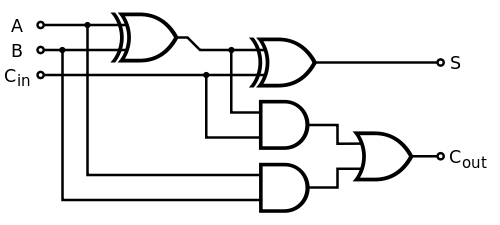
\includegraphics[width=80mm]{Lab3/figures/fulladder.png}
	\caption{Circuit for a 1-bit full adder}
	\label{fig:fulladder}
\end{figure}

Now that you have a working 1-bit full adder, implement a 4-bit ripple carry adder that sums the binary numbers "0110" and "0101." A block diagram for the 4-bit ripple carry adder is shown in Figure \ref{fig:fourbitripple}. Verify your results by creating a waveform and simulating the circuit.

\begin{figure}[H]
	\centering
	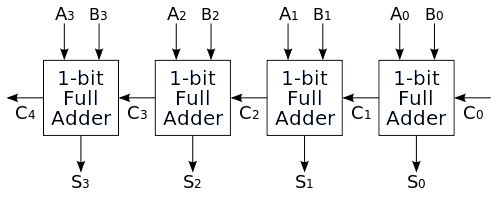
\includegraphics[width=100mm]{Lab3/figures/fourbitripple.png}
	\caption{4-bit ripple carry adder block diagram}
	\label{fig:fourbitripple}
\end{figure}

\subsubsection{Full Adder Based ALU}
The block diagram in Figure \ref{fig:fulladderalu} is an example of how the regular 1-bit full adder can be manipulated to implement additional functionality. For this activity, you must build VHDL code that implements a 4-bit complex adder ALU, the list of instructions can be found in Table \ref{tab:adderaluop}.

\begin{figure}[H]
	\centering
	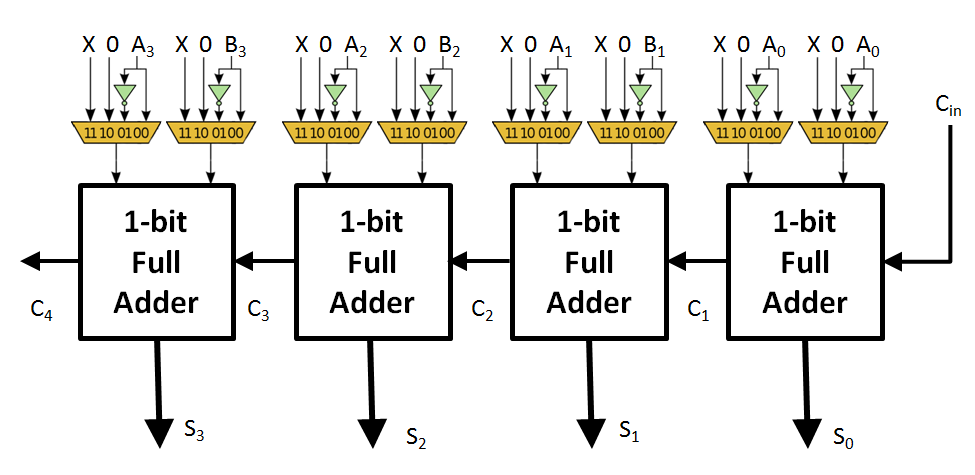
\includegraphics[width=150mm]{Lab3/figures/fulladderalu.png}
	\caption{Block diagram for a 4-bit ripple carry adder ALU with 12 operations}
	\label{fig:fulladderalu}
\end{figure}

After writing and testing your VHDL code, upload it on the DE2-115 FPGA Development board. Connect the inputs {\bf A3-A0} to SW3 - SW0 and the inputs {\bf B3-B0} to SW4(7)- SW(4). Connect the select lines for the {\bf A} multiplexer to SW(8) and SW(9) while the select lines for {\bf B} should connect to SW10 and SW11. Lastly, the carry in input should connect to SW12. Display inputs {\bf A} and {\bf B} in hexadecimal on HEX7 and HEX5, respectively and the output {\bf S}, on HEX3. If the result over-flows display {\bf C$_4$} on LEDG0. If the result is zero turn on LEDR1. Test and verify all twelve operations are correct and make a table that includes the values for {\bf A}, {\bf B}, {\bf S}, {\bf C$_4$}, and {\bf Zero} for each operation.

\begin{table}[H]
	\centering
	\caption{List of opperations for the adder based ALU}
	\begin{tabular}{ | c | c | c | c | }
		\hline                        
 		\bf A$_i$ & \bf B$_i$ & \bf Carry In & \bf Result \\ \hline
 		Set to 0 & Set to 0 & 0 & 0 \\ \hline
 		Set to 0 &  Set to 0 & 1 & 1 \\ \hline
 		A &  Set to 0 & 0 & A \\ \hline
 		Set to 0 & B  & 0  & B  \\ \hline
 		A & Set to 0 & 1 & A $+$ 1 \\ \hline
 		Set to 0 & B & 1 & B $+$ 1 \\ \hline
 		A & B & 0 & A $+$ B \\ \hline
 		Set to invert & B & 1 & B $-$ A \\ \hline
 		Set to invert & Set to 0 & 0 & $\overline{A}$ \\ \hline
 		Set to invert & Set to 0 & 1 & $-$A \\  \hline
		Set to 0 & Set to invert & 0 & $\overline{B}$ \\ \hline
 		Set to 0 & Set to invert & 1 & $-$B \\ 
 		\hline
	\end{tabular}
	\label{tab:adderaluop}
\end{table}

When you complete building the VHDL upload your code to the FPGA board. Test and verify all twelve operations are correct.

\subsection{Lab Report}
Your lab report submission should break down as follows:
\begin{itemize}
	\item Extract from the fpga lab folder the VHDL file from each project, upload each of them to the Sakai Assignment page. Ex: part1.vhdl and part2.vhdl
	\begin{itemize}
		\item Make sure that your code is well commented.
	\end{itemize}
	\item Waveforms for the Half Adder and Full Adder.
	\item For Part 3 after compilation go to Tools > Netlist Viewers > RTL Viewer. Print a pdf of this page and discuss what you see.
	\item Your report should include a one page discussion on the number of pins used and your table from part 3.
\end{itemize}
